\documentclass{article}
\usepackage{amsmath}
\usepackage{mathtools}
\usepackage{gensymb}
\usepackage[a4paper,inner=1.5cm,outer=1.5cm,top=2cm,bottom=0.5cm]{geometry} 
\usepackage{xcolor}                    
\usepackage{tikz}                           
\usepackage{multicol}
\usepackage{pgfplots}
\usetikzlibrary{calc}
\usetikzlibrary{intersections}
\usetikzlibrary{intersections,calc,angles,quotes}
\usetikzlibrary{shapes,arrows,positioning,decorations.pathreplacing,calc}
\usetikzlibrary{calc,angles,positioning,intersections,quotes,decorations.markings}
\usepackage{tkz-euclide}
\usetikzlibrary{backgrounds}
\usetikzlibrary{calc,through}
\usetikzlibrary{angles}
\usetikzlibrary{fadings}
\usetikzlibrary{shapes.geometric}
\usetikzlibrary{shapes.symbols}
\usepackage{draftwatermark}
\usepackage{mathptmx}

\SetWatermarkText{\textcolor{black!30}{Mathema Shukur}}
\SetWatermarkFontSize{2 cm}
\usepackage[utf8]{inputenc}
\usepackage{fontspec}

\setmainfont{[Kalpurush.ttf]}
\newfontface{\en}{[Arial.ttf]} %%this is optional, if you want to use a secondary font. Any english font is supported
\newlength\Radius
\setlength\Radius{4cm}
\begin{document} 
	\Large
	\textcolor{red}{Welcome To} 
	\\
	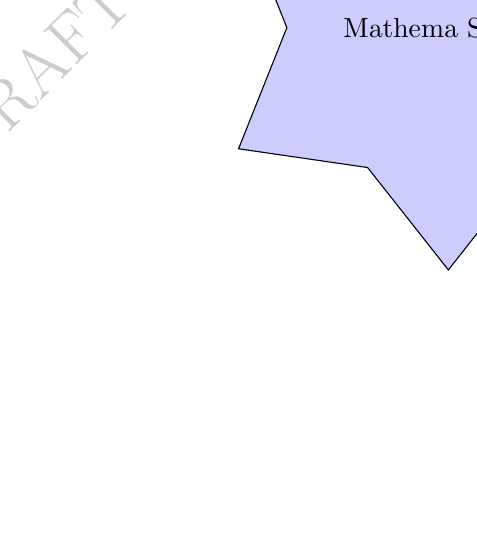
\begin{tikzpicture}
		\tikz \node [fill=blue!20,star,star points=6,draw] {Mathema Shukur };
	\end{tikzpicture}
	\\
	যাদের জন্যে প্রযোজ্যঃ  	\textcolor{magenta}{একাদশ ও দ্বাদশ শ্রেণীর শিক্ষার্থী} \\
	বিষয়ঃ \textcolor{magenta}{উচ্চতর গণিত ১ম পত্র} \\
	অধ্যায়ঃ \textcolor{magenta}{৩-সরলরেখা}\\ 
	Subtopicঃ  \textcolor{magenta}{ সমান্তরাল নয় এমন দুইটি সরলরেখার অন্তর্ভুক্ত কোণ নির্ণয় }\\
	\\
	\begin{tikzpicture}[transform shape,scale=1]
		\draw [-latex,thick](-6,0) -- (6,0) node[right] {$x$} coordinate(x axis);
		\draw [-latex,thick](0,-3) -- (0,7) node[above] {$y$} coordinate(y axis);
		\fill[black] (0,0) circle (1 mm);
		\node at (0.3,-0.3) {$\textcolor{purple}{O}$};	
		\node at (-1,0.3) {$\textcolor{blue}{\theta_2}$};	
		\node at (-4,-2) {$\textcolor{blue}{C}$};	
		\node at (5,5) {$\textcolor{blue}{D}$};	
		\node at (1,0.3) {$\textcolor{green}{\theta_1}$};	
			\node at (-1,-2) {$\textcolor{green}{A}$};	
				\node at (3,5.3) {$\textcolor{green}{B}$};	
		\node at (1.4,2.2) {$\textcolor{red}{\varphi}$};	
			\node at (5,3) {$\textcolor{red}{\varphi}+\textcolor{blue}{\theta_2}=\textcolor{green}{\theta_1}$};	
				\node at (5,2) {$\textcolor{red}{\varphi}=\textcolor{green}{\theta_1}-\textcolor{blue}{\theta_2}$};	
		\draw[very thick,green] (-1,-3)--(3,5);	
		\draw[very thick,blue] (-6,-3)--(6,6);	
	\end{tikzpicture}
\\
$AB$ সরলরেখার ঢাল $m_1=\tan \theta_1$,\quad $CD$ সরলরেখার ঢাল  $m_2=\tan \theta_2$\\ 
\vspace{3cm}
\begin{multicols}{2}
	\begin{align*}
	\boxed{\theta_1>\theta_2}&\\
	\\
	m_1&=\tan \theta_1\\
	\\
	m_2&=\tan \theta_2\\
	\\
	\tan \varphi &=\tan(\theta_1-\theta_2)\\
	\\
	\tan \varphi 	&=\frac{\tan \theta_1-\tan \theta_2}{1+\tan \theta_1\,\,\tan \theta_2}\\
	\\
	\tan \varphi 	&=\frac{m_1-m_2}{1+m_1\,\,m_2}
\end{align*}
\\
\begin{align*}
	\boxed{\theta_2>\theta_1}&\\
	\\
	m_1&=\tan \theta_1\\
	\\
	m_2&=\tan \theta_2\\
	\\
	\varphi&=(\theta_2-\theta_1)=-(\theta_1-\theta_2)\\
	\\
	\tan \varphi &=-\tan(\theta_1-\theta_2)\\
	\\
	\tan \varphi 	&=-\frac{\tan \theta_1-\tan \theta_2}{1+\tan \theta_1\,\,\tan\theta_2}\\
	\\
	\tan \varphi 	&=-\frac{m_1-m_2}{1+m_1\,\,m_2}
\end{align*}
\end{multicols}
$\tan \varphi$ এর মান ধনাত্মক হলে রেখাদ্বয়ের মধ্যবর্তীকোণ সুক্ষকোণ হবে\\
\\
$\tan \varphi$ এর মান ঋণাত্মক হলে রেখাদ্বয়ের মধ্যবর্তীকোণ স্থূলকোণ হবে\\
\\
Working Formula\\
\\
\boxed{	\tan \varphi 	=\pm \frac{m_1-m_2}{1+m_1\,\,m_2}}\\
\\ 
যশোর বোর্ড-২০২১\\ 
$4x-3y+12=0$ এবং $3x+4y-10=0$ রেখা দুইটির মধ্যবর্তী কোণ নির্ণয় কর\\ 
	\\ 
\textcolor{blue}{$ax+by+c=0$ সরলরেখার ঢাল  $m=-\frac{a}{b}$}\\
\\
$4x-3y+12=0$  সরলরেখার ঢাল $m_1=-\frac{4}{(-3)}=\frac{4}{3}$\\
\\
 $3x+4y-10=0$  সরলরেখার ঢাল $m_2=-\frac{3}{4}=-\frac{3}{4}$\\
\\
ধরি, 	$4x-3y+12=0$ এবং $3x+4y-10=0$ রেখাদ্বয়ের মধ্যবর্তী কোণ $\varphi$\\
\\
\begin{align*}
	\tan \varphi 	&=\pm \frac{m_1-m_2}{1+m_1\,\,m_2}\\
	\\
	\tan \varphi 	&=\pm \frac{\frac{4}{3}-\left(-\frac{3}{4}\right)}{1+\left(\frac{4}{3}\right)\left(-\frac{3}{4}\right)}\\
	\\
	\tan \varphi 	&=\pm \frac{\frac{4}{3}+\frac{3}{4}}{1-1}\\	
	\\
	\tan \varphi&=\pm \frac{\frac{25}{12}}{0}\\
	\\
	\varphi&=90\degree
\end{align*}
\\
	\begin{tikzpicture}[transform shape,scale=1]
	\draw [-latex,thick](-6,0) -- (6,0) node[right] {$x$} coordinate(x axis);
	\draw [-latex,thick](0,-4) -- (0,8) node[above] {$y$} coordinate(y axis);
	\fill[black] (0,0) circle (1 mm);
	\node at (0.3,-0.3) {$\textcolor{purple}{O}$};	
	\node at (-3,6.5) {$\textcolor{blue}{3x+4y-10=0}$};	
	\node at (3.5,6) {$\textcolor{green}{4x-3y+12=0}$};	
	\node at (-1.5,3) {$\textcolor{red}{90\degree}$};	
	\draw[very thick,green] (-6,-4)--(3,8);	
	\draw[very thick,blue] (-6,7)--(6,-2);	
\end{tikzpicture}
\\
দিনাজপুর বোর্ড-২০২১\\
$y=2x+3$ এবং $3x-y+5=0$ রেখা দুইটির মধ্যবর্তী কোণ নির্ণয় কর\\ 
\\
	\\ 
\textcolor{blue}{$ax+by+c=0$ সরলরেখার ঢাল  $m=-\frac{a}{b}$}\\
\\
$2x-y+3=0$  সরলরেখার ঢাল $m_1=-\frac{2}{(-1)}=2$\\
\\
$3x-y+5=0$  সরলরেখার ঢাল $m_2=-\frac{3}{(-1)}=3$\\
\\
ধরি, $y=2x+3$ এবং $3x-y+5=0$ রেখাদ্বয়ের মধ্যবর্তী কোণ $\varphi$\\
\\
\begin{align*}
	\tan \varphi 	&=\pm \frac{m_1-m_2}{1+m_1\,\,m_2}\\
	\tan \varphi 	&=\pm \frac{2-3}{1+(2)(3)}\\
	\tan \varphi 	&=\pm \frac{-1}{7}\\	
	\tan \varphi&=\pm \frac{1}{7}\\	
	\varphi&=8.13\degree,\qquad 171.87\degree
\end{align*}
\\
\begin{tikzpicture}[transform shape,scale=1]
	\draw [-latex,thick](-6,0) -- (3,0) node[right] {$x$} coordinate(x axis);
	\draw [-latex,thick](0,-4) -- (0,8) node[above] {$y$} coordinate(y axis);
	\fill[black] (0,0) circle (1 mm);
	\node at (0.3,-0.3) {$\textcolor{purple}{O}$};	
	\node at (-2,6) {$\textcolor{blue}{3x-y+5=0}$};	
	\node at (3,5) {$\textcolor{green}{2x-y+3=0}$};	
	\node at (-0.7,2) {$\textcolor{red}{8.13\degree}$};	
	\draw[very thick,green] (-4,-4)--(1,5);	
	\draw[very thick,blue] (-4,-6)--(1,8);	
\end{tikzpicture}
\\
	(1) দিনাজপুর বোর্ড-২০১৯\\
	$x-2y-5=0$ ও $2x+4y-1=0$ রেখাদ্বয়ের মধ্যবর্তী কোণ নির্ণয় কর। \\ 
	\\ 
	\textcolor{blue}{$ax+by+c=0$ সরলরেখার ঢাল  $m=-\frac{a}{b}$}\\
	\\
		$x-2y-5=0$  সরলরেখার ঢাল $m_1=-\frac{1}{(-2)}=\frac{1}{2}$\\
		\\
	$2x+4y-1=0$  সরলরেখার ঢাল $m_2=-\frac{2}{4}=-\frac{1}{2}$\\
		\\
		ধরি, 	$x-2y-5=0$ ও $2x+4y-1=0$ রেখাদ্বয়ের মধ্যবর্তী কোণ $\varphi$\\
		\\
		\begin{align*}
		\tan \varphi 	&=\pm \frac{m_1-m_2}{1+m_1\,\,m_2}\\
		\\
			\tan \varphi 	&=\pm \frac{\frac{1}{2}-\left(-\frac{1}{2}\right)}{1+\left(\frac{1}{2}\right)\left(-\frac{1}{2}\right)}\\
			\\
			\tan \varphi 	&=\pm \frac{\frac{1}{2}+\frac{1}{2}}{1-\frac{1}{4}}\\	
			\\
			\tan \varphi&=\pm \frac{4}{3}\\
			\\
			\varphi&=53.13\degree,\qquad 126.87\degree
		\end{align*}
	\\
	\\
	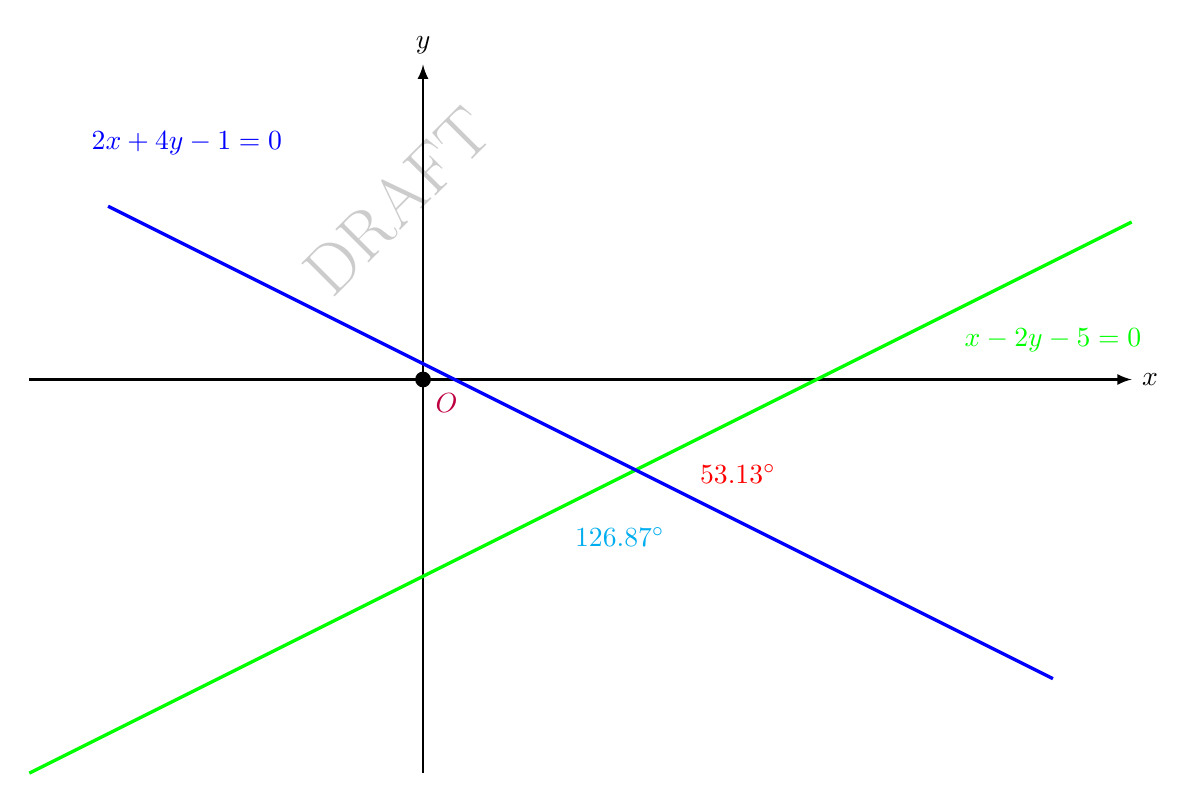
\begin{tikzpicture}[transform shape,scale=1]
		\draw [-latex,thick](-5,0) -- (9,0) node[right] {$x$} coordinate(x axis);
		\draw [-latex,thick](0,-5) -- (0,4) node[above] {$y$} coordinate(y axis);
		\fill[black] (0,0) circle (1 mm);
		\node at (0.3,-0.3) {$\textcolor{purple}{O}$};	
		\node at (-3,3) {$\textcolor{blue}{2x+4y-1=0}$};	
		\node at (8,0.5) {$\textcolor{green}{x-2y-5=0}$};	
		\node at (4,-1.2) {$\textcolor{red}{53.13\degree}$};	
			\node at (2.5,-2) {$\textcolor{cyan}{126.87\degree}$};
		\draw[very thick,green] (-5,-5)--(9,2);	
		\draw[very thick,blue] (-4,2.2)--(8,-3.8);	
	\end{tikzpicture}
	\\
	(ঢাকা বিশ্ববিদ্যালয় ভর্তি পরীক্ষা-২০১৮-২০১৯)\\
	$y=b$ এবং $\sqrt{3}x-y+1=0$	রেখাদ্বয়ের অন্তর্ভুক্ত সুক্ষকোণের মান নির্ণয় কর\\
	\\
		$y=b$ রেখাটি $x-$ অক্ষের সমান্তরাল \\
		\\
		 $\sqrt{3}x-y+1=0$ রেখাটি 	$y=b$ রেখার সাথে যে কোণ উৎপন্ন করে , $x$ অক্ষের সাথে একই কোণ উৎপন্ন করে। \\
		 \\
	 $\sqrt{3}x-y+1=0$	  সরলরেখার ঢাল $m_1=-\frac{\sqrt{3}}{(-1)}=\sqrt{3}$\\
	 \\ 
	 $\tan \theta=\sqrt{3},\qquad \theta=60\degree$\\
	 \\
	 \begin{tikzpicture}[transform shape,scale=1]
	 	\draw [-latex,thick](-5,0) -- (9,0) node[right] {$x$} coordinate(x axis);
	 	\draw [-latex,thick](0,-5) -- (0,4) node[above] {$y$} coordinate(y axis);
	 	\fill[black] (0,0) circle (1 mm);
	 	\node at (0.3,-0.3) {$\textcolor{purple}{O}$};	
	 	\node at (-5,-2) {$\textcolor{blue}{y=b}$};	
	 	\node at (3,3) {$\textcolor{green}{\sqrt{3}x-y+1=0}$};	
	 	\node at (-0.2,0.5) {$\textcolor{red}{60\degree}$};	
	 		\node at (-1,-1.5) {$\textcolor{red}{60\degree}$};	
	 	\draw[very thick,green] (2,4.5)--(-3,-4);	
	 	\draw[very thick,blue] (-4,-2)--(4,-2);	
	 \end{tikzpicture}
 \\
		(ঢাকা বিশ্ববিদ্যালয় ভর্তি পরীক্ষা-২০১৭-২০১৮)\\
	$x=a$ এবং $\sqrt{3}x-y+1=0$	রেখাদ্বয়ের অন্তর্ভুক্ত সুক্ষকোণের মান নির্ণয় কর\\
 \\
 	$x=a$  রেখাটি $y-$ অক্ষের সমান্তরাল অর্থাৎ  $x$ অক্ষের উপর লম্ব \\
\\
 $\sqrt{3}x-y+1=0$	  সরলরেখার ঢাল $m_1=-\frac{\sqrt{3}}{(-1)}=\sqrt{3}$\\
 \\ 
 $\tan \theta=\sqrt{3},\qquad \theta=60\degree$\\
 \\
  $\sqrt{3}x-y+1=0$	 রেখাটি $x-$ অক্ষের ধনাত্মক দিকের সাথে $60\degree$ কোণ তৈরী করে \\
  \\ 
  	$x=a$  রেখাটি $x-$ অক্ষের সাথে $90\degree$ কোণ তৈরী করে \\
  	\\ 
 	$x=a$ এবং $\sqrt{3}x-y+1=0$	রেখাদ্বয়ের অন্তর্ভুক্ত সুক্ষকোণের মান $\alpha$\\
 	\\
\begin{tikzpicture}[transform shape,scale=1]
	\draw [-latex,thick](-5,0) -- (9,0) node[right] {$x$} coordinate(x axis);
	\draw [-latex,thick](0,-5) -- (0,4) node[above] {$y$} coordinate(y axis);
	\fill[black] (0,0) circle (1 mm);
	\node at (0.3,-0.3) {$\textcolor{purple}{O}$};	
	\node at (1.7,-2) {$\textcolor{blue}{x=a}$};	
	\node at (3,3) {$\textcolor{green}{\sqrt{3}x-y+1=0}$};	
	\node at (-0.2,0.5) {$\textcolor{red}{60\degree}$};	
	\node at (0.7,1.8) {$\textcolor{red}{\alpha}$};	
		\node at (0.7,0.3) {$\textcolor{red}{90\degree}$};	
	\draw[very thick,green] (2,4.5)--(-3,-4);	
	\draw[very thick,blue] (1,5)--(1,-5);	
\end{tikzpicture}
\\
ত্রিভুজের তিন কোণের সমষ্টি দুই সমকোণ $(180\degree)$\\
\\
$\alpha+60\degree+90\degree=180\degree$\\
\\
$\alpha=30\degree$
\end{document}